\documentclass[aspectratio=169]{beamer}
\setbeamertemplate{navigation symbols}{}

%Compile with !pdflatex % and !biber slides
\usepackage[backend=biber,style=chem-acs]{biblatex}
\addbibresource{pres.bib}
\AtBeginEnvironment{frame}{\setcounter{footnote}{0}}
\setbeamertemplate{footline}[frame number]

\usepackage{graphicx}
\usepackage{amsmath}
\usepackage{braket}
\usepackage{verbatim}

\renewcommand\multicitedelim{\addsemicolon\space}
\newcommand\blfootnote[1]{%
  \begingroup
  \renewcommand\thefootnote{}\footnote{#1}%
  \addtocounter{footnote}{-1}%
  \endgroup
}

\title{Introduction to a Couple of Things}
\author{Harper Grimsley}
%\institute{Mayhall Group, Virginia Tech}
\date{TBD}

\begin{document}

\frame{\titlepage}

\begin{frame}
	\frametitle{Why Quantum Chemistry is Hard}
	\begin{itemize}[<+->]
		\item Schr{\"o}dinger says to solve:
			\begin{equation}\nonumber
			\mathcal{H}\ket{\Psi} = E\ket{\Psi}
			\end{equation}
		\item $\ket{\Psi}$ includes exponentially many configurations- exponential memory to store $\ket{\Psi}$
		\item Dimension of $\mathcal{H}$ scales exponentially- diagonalizing it requires exponential time
	\end{itemize}
\end{frame}

\begin{frame}
	\frametitle{Quantum Computers and Storage}
	\begin{itemize}[<+->]
		\item Quantum registers of $N$ qubits exist in linear combinations of $2^N$ configurations
		\item Jordan-Wigner maps all configurations of $N$ spinorbitals to $N$ qubits
		\item E.g. H$_2$ in minimal basis:
			\begin{equation}\nonumber
				c_0\ket{\phi_0} + c_{0\bar{0}}^{1\bar{1}}\ket{\phi_{0\bar{0}}^{1\bar{1}}}\rightarrow c_{\uparrow\uparrow\downarrow\downarrow}\ket{\uparrow\uparrow\downarrow\downarrow}+c_{\downarrow\downarrow\uparrow\uparrow}\ket{\downarrow\downarrow\uparrow\uparrow}
			\end{equation}
		\item This is just a 4-electron spin state: one for each spinorbital
	        \item Number of qubits scales linearly with system size!
	\end{itemize}
\end{frame}

\begin{frame}
	\frametitle{Quantum Phase Estimation\footfullcite{abrams_quantum_1999}}
	\begin{itemize}[<+->]
		\item Reformulate as finding eigenvalue of a unitary
			\begin{align}\nonumber
				&\mathcal{H}\ket{\Psi}=E\ket{\Psi}\\\rightarrow &e^{i\mathcal{H}}\ket{\Psi} = e^{iE}\ket{\Psi}\equiv e^{2\pi i\phi}\ket{\Psi}\nonumber
			\end{align}
		\item Quantum computer can find $\phi$:
			\begin{figure}
				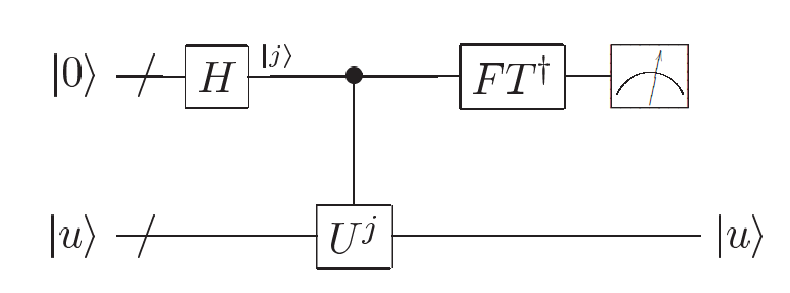
\includegraphics[width=.45\textwidth]{pea_overall.png}%
				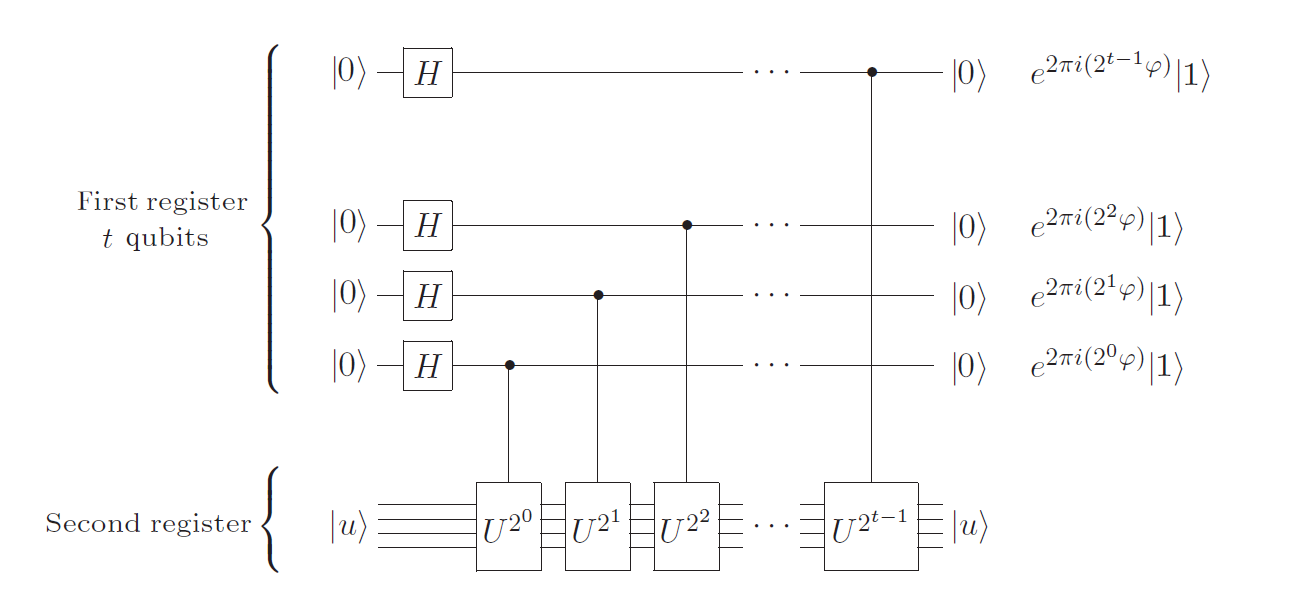
\includegraphics[width=.45\textwidth]{pea_1.png}%
			\caption{Nielsen and Chuang, 2011}
			\end{figure}
        \end{itemize}
\end{frame}



\begin{frame}
	\frametitle{Qubitization and Block Encoding \footfullcite{low_hamiltonian_2019}}
	\begin{itemize}[<+->]
	\item Time evolution operator is $e^{-i\mathcal{H}t}$
	\item How can we simulate this without Trotterization?
	\item One strategy is to approximate this function of $\mathcal{H}$ as a non-unitary polynomial
	\item Construction of non-unitary operators is also desirable for, e.g., open systems	
	\end{itemize}

\end{frame}

\begin{frame}
	\frametitle{Block-Encoding}
	\begin{itemize}[<+->]
	\item Quantum computers can only execute unitary operators
	\item We can cheat by embedding a non-unitary operator in a unitary one
	\begin{equation}
	\hat{U} = \begin{pmatrix}\mathcal{H} & * \\ * & *\end{pmatrix}
	\end{equation}
	\item For ancilla state $\ket{G}_a$ and system state $\ket{\psi}_s$
	\begin{align}
		\nonumber \hat{U}\ket{G}_a\ket{\psi}_s &= \ket{G}_a\mathcal{H}\ket{\psi}_s+\sqrt{1-\braket{\psi|\mathcal{H}^2|\psi}}\ket{G_\psi^{\perp}}_{as}\\
		\nonumber (\bra{G}_a\otimes \mathbf{I})\ket{G_\psi^{\perp}}_{as}&= 0
	\end{align}
	\item Spectral Form:
		\begin{align}
		\nonumber\hat{U}\ket{G}\ket{\lambda}&\equiv\hat{U}\ket{G_\lambda}\\
		\nonumber&=\lambda{G_\lambda}+\sqrt{1-|\lambda|^2}\ket{G_\lambda^{\perp}}
		\end{align}
	\end{itemize}
\end{frame}

\begin{frame}
	\frametitle{Constructing $\hat{U}$: Linear Combination of Unitaries\footfullcite{childs_hamiltonian_2012}}
	\begin{itemize}[<+->]
		\item Every Hamiltonian can be written as a linear combination of d unitaries:
		\begin{equation}\nonumber
		\mathcal{H} = \sum_{j=1}^d \alpha_j \hat{U}_j
		\end{equation}
		\item It can be shown that we can always use:
		\begin{align}
			\nonumber \ket{G} &= \sum_{j=1}^d\sqrt{\alpha_j/||\boldsymbol{\alpha}||_1}\ket{j}_a\\
			\nonumber \hat{U} &= \sum_{j=1}^d\ket{j}\bra{j}_a\otimes\hat{U}_j
		\end{align}
		\item This gives 
		\begin{equation}
			\mathcal{H} = ||\boldsymbol{\alpha}||_1(\bra{G}_a\otimes \mathbf{I}_s)\hat{U}(\ket{G}_a\otimes\mathbf{I})
		\end{equation}
	\end{itemize}
\end{frame}

\begin{frame}
	\frametitle{Simple Example of Block-Encoding Using LCUs}
	\begin{itemize}[<+->]
	\item Consider a special case of the 2-qubit Heisenberg Hamiltonian:
	\begin{equation}\nonumber
		\mathcal{H} = \hat{X}\hat{X}+\hat{Z}\hat{Z}
	\end{equation}
	\item This is already a sum of unitaries, so we choose
	\begin{align}
	\nonumber \ket{G} &= \frac{1}{\sqrt{2}}(\ket{0}+\ket{1})\equiv{\ket{+}}\\
	\nonumber \hat{U} &= \ket{0}\bra{0}\hat{X}\hat{X}+\ket{1}\bra{1}\hat{Z}\hat{Z}
	\end{align}
	\item With some algebra, we get
	\begin{equation} \nonumber
		\hat{U}\ket{G}\ket{\psi}_s = \frac{1}{2}\ket{+}\mathcal{H}\ket{\psi}_s + \frac{1}{2}\ket{-}(\hat{X}\hat{X}-\hat{Z}\hat{Z})\ket{\psi}_s
	\end{equation}
	\item We just measure the first qubit in the $\ket{+}/\ket{-}$ basis, and when we get $\ket{+}$, we know we have (up to a normalization constant) $\mathcal{H}\ket{\psi}_s$ on the other qubits!
	\end{itemize}
\end{frame}

\begin{frame}
	\frametitle{Qubitization}
	\begin{itemize}[<+->]
	\item Our original goal was to build functions of $\mathcal{H}$
	\item Does $\hat{U}^2$ enact $\mathcal{H}^2$ on the system qubits?
	\item No- Higher powers of $\hat{U}$ leave the $SU(2)$ subspace: span$\{\ket{G}_\lambda,\hat{U}\ket{G_\lambda}\}$
	\item We can fix this ``leakage'' by replacing $\hat{U}$ with an \textit{iterate} $\hat{W}$
		\begin{align}
			\nonumber \hat{W}&=\oplus_{\lambda}\begin{pmatrix} \lambda & -\sqrt{1-|\lambda|^2} \\ \sqrt{1-|\lambda|^2} & \lambda\end{pmatrix}_\lambda\\
		\nonumber &=\oplus e^{-i\hat{Y}_\lambda \arccos(\lambda)}
		\end{align}
	\item This is called qubitization because it breaks up the operator into a direct sum of SU(2) unitaries
	\end{itemize}
\end{frame}

\begin{frame}
	\frametitle{Qubitization Recipe}
	\begin{itemize}[<+->]
		\item We know how to get a block-encoded operator $\hat{U}$ and ancilla state $\ket{G}$ with LCUs, but how do we get $\hat{W}$?
	\item The math is boring, but there is a universal construction of this as well:
	\begin{align}
		\nonumber \ket{G'} &= \ket{+}\ket{G}\\
		\nonumber \hat{W} &= \ket{1}\bra{0}\otimes\hat{U} + \ket{0}\bra{1}\otimes\hat{U}^{\dagger}
	\end{align}
	\item Note that this na{\"i}ve approach requires an additional ancilla qubit
	\end{itemize}
\end{frame}

\begin{frame}
	\frametitle{Payoff: Quantum Signal Processing \footfullcite{low_optimal_2017}}
	\begin{itemize}[<+->]
	\item We originally promised the ability to implement functions of $\mathcal{H}$- we now have the tools to accomplish this
	\item Quantum Signal Processing manipulates $\hat{W}$ to construct a block-encoded function of $\mathcal{H}$:
	\begin{equation}\nonumber
	f(\mathcal{H}) = A(\mathcal{H})+iB(\mathcal{H})
	\end{equation}
	where $A$ and $B$ are real-valued polynomials
	\item We will treat this as a black box
	\end{itemize}
\end{frame}

\begin{frame}
	\frametitle{Application: Time Evolution Operator}
	\begin{itemize}[<+->]
	\item Spectral form of Jacobi-Anger Expansion:
		\begin{equation}\nonumber
			e^{-i\lambda t} = J_0(t) + 2\sum_{\text{even }k >0}^{\infty}(-1)^{k/2}J_k(t)T_k(\lambda) + 2i\sum_{\text{odd }k >0}^{\infty}(-1)^{(k-1)/2}J_k(t)T_k(\lambda)
		\end{equation}
	\item Approximate as $A(\lambda)+iB(\lambda)$ where
	\begin{align}
		\nonumber A(\lambda) &=  J_0(t) + 2\sum_{\text{even }k >0}^{Q}(-1)^{k/2}J_k(t)T_k(\lambda)\\
		\nonumber B(\lambda) &=  2i\sum_{\text{odd }k >0}^{Q}(-1)^{(k-1)/2}J_k(t)T_k(\lambda)
	\end{align}
	\item Put all the pieces together:
		\begin{equation}\nonumber
			\hat{H}\rightarrow\hat{U}\rightarrow\hat{W}\rightarrow A(\mathcal{H})+iB(\mathcal{H})\approx e^{-i\mathcal{H}t}
		\end{equation}
	\end{itemize}
\end{frame}

\begin{frame}
	\frametitle{Summary of Block-Encoding and Quantum Signal Processing}
	\begin{itemize}[<+->]
	\item These tools can be used to construct non-unitary operators for quantum computing
	\item E.g. approximate non-Trotterized time evolution operator
	\item Lots of room to do this in a smarter, problem-specific way
	\item E.g., unitary decompositions of $\mathcal{H}$ are non-unique and require different numbers of ancilla qubits
	\end{itemize}
\end{frame}

\begin{frame}
\begin{center}
	\huge{Thank you for your attention!}
\end{center}
\end{frame}
\end{document}
